\chapter{Design of Verlixir} \label{chap:design}
This chapter provides an in-depth insight into the design decisions that were made during the development of Verlixir and LTLixir. The chapter will begin by providing a high-level overview of where the relevant components fit into the toolchain, as well as providing an architectural overview of the tool. Section \ref{sec:specification_language} will discuss the design of LTLixir, section \ref{sec:modelling_elixir_programs} will describe the main techniques Verlixir applies in the analysis and modelling of a specification. Finally, section \ref{sec:simulation_verification} will describe the derivations of the outputs generated by Verlixir.  
\section{Verlixir Toolchain} \label{sec:toolchain}
We will now introduce where the new tools fit into the grater toolchain. Figure \ref{fig:high_level} shows a high-level overview of the toolchain. Given an LTLixir specification, there are two main paths to be taken. Either, the underlying elixir program can be compiled and ran on the ERTS as normal, or the program can be modelled by Verlixir and verified with Spin.
\begin{figure}[H]
    \centering
    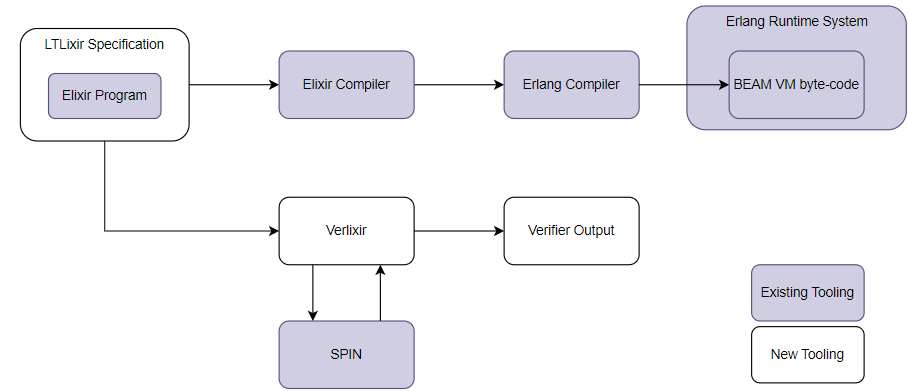
\includegraphics[width=0.8\textwidth]{images/high_level_system.png}
    \caption{High-level overview of the verifiable Elixir toolchain.}
    \label{fig:high_level}
\end{figure}
Figure \ref{fig:low_level} provides an in-depth insight into the architecture underlying Verlixir.
\begin{figure}[H]
    \centering
    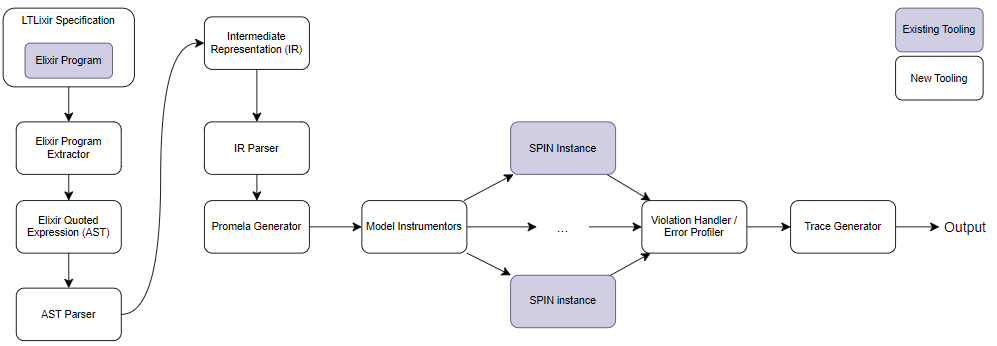
\includegraphics[width=1\textwidth]{images/low_level_system.png}
    \caption{Verlixir design.}
    \label{fig:low_level}
\end{figure}
Before we provide an in-depth discussion on the design of Verlixir, we will summarise the components of the tool.
\begin{itemize}
    \item \textbf{LTLixir Specification}: Specification of an Elixir program to be parsed by Verlixir.
    \item \textbf{Elixir Extractor}: Converts the Elixir program into a quoted expression.
    \item \textbf{AST Parser}: Parses the quoted expression into an intermediate representation.
    \item \textbf{IR Parser}: Parses the intermediate representation, collecting relevant information for the model generator.
    \item \textbf{Promela Generator}: Writes a promela model from the intermediate representation.
    \item \textbf{Model Instrumentors}: Instruments the model for appropriate verification (depending on system and user requirements).
    \item \textbf{Violation Handler}: Handles the output of the model checker by mapping violations back to the original Elixir program.
    \item \textbf{Trace Generator}: Generates an error trace from the mapped Elixir violations.
\end{itemize}
\section{Specification Language} \label{sec:specification_language}
LTLixir is a specification language that can be used to reason about the time and change of an Elixir system using LTL formulae. An LTLixir specification is the input to Verlixir and is used to guide the model generation process. Primarily, LTLixir supports a restricted subset of Elixir, with additional constructs to support specification properties. This section will primarily discuss the design decisions behind the additional constructs. For information on how LTLixir is transformed in model generation, see section \ref{sec:supporting_ltl}.
\\ \\
\subsubsection{Specification Constructs}
There is only one construct in LTLixir that is imperative to successfully interact with the simulator and verifier. \texttt{@vae\_init} is an attribute that is assigned a value, $v \in \{true, false\}$. The attribute is treated by the Elixir compiler as a regular attribute, so will not cause issues when running within the ERTS. Importantly, for Verlixir, it is used to determine an entry point to the system.
\\ \\
\subsubsection{Attributes}
All the remaining constructs of the specification are optional to the verification of the system. Similarly to the \texttt{@vae\_init} attribute, \texttt{@spec}, \texttt{@ltl} and \texttt{@params} are all attributes that are assigned values. The \texttt{@spec} is already well-defined in the Elixir language, although it is noted that type specifications do not instrument Elixir programs in any way. Instead, \texttt{@spec} can be used by analysis tools that run on Elixir programs. In our case, we reduce the possible type specifications which can be defined. There are two key differences between an Elixir type specification and an LTLixir type specification. Firstly, LTLixir does not support the use of custom types introduced through the \texttt{@type} attribute. Only a set of primitive types are accepted within a specification: $\{integer(), boolean(), atom()\}$.
\\ \\
The second restriction applied by LTLixir is the return type \texttt{:ok}. This atom is reserved in type specifications to mark functions whose return values are never matched on. The actual return type of the function is not relevant in this instance as an agreement is made with the developer that the function will never be matched. The \texttt{@ltl} attribute assigns a string value. This string value must follow the imposed rules on LTL formula by LTLixir. Namely, it must follow a formula of the form introduced in section \ref{sec:verifiable} with the additional allowance of the Elixir constructs identifiers, boolean operations and binary operations. All the identifiers must be well-defined within the scope of the function and should not be declared in a nested child scope within the function. The final attribute LTLixir supports is \texttt{@params}. \texttt{@params} is assigned a tuple of atoms. Similarly to the \texttt{@ltl} attribute, the tuple should consist of atom identifiers from the function scope.
\\ \\
\subsubsection{Verifiable Constructs}
The next construct we will discuss is \texttt{defv}. The \texttt{defv} construct no longer `annotates' information about the specification of a function, instead it is directly inlined into the function definition. \texttt{defv} defines a `verifiable function'. A verifiable function is a third function type definition alongside \texttt{def} and \texttt{defp}. Semantically, it acts similar to \texttt{def}, as it is a public function that can be accessed from external module calls. The \texttt{defv} construct is what Elixir refers to as a macro. A macro is used to extend the Elixir syntax through metaprogramming. The macro introduces two new tuples to the arguments of the quoted expression representing the function. Syntactically, these tuples can be defined using the terms \texttt{pre:} and \texttt{post:} in the function declaration, before the body of the function.
\begin{lstlisting}[language=Elixir, xleftmargin=.1\linewidth, caption={Example of the \texttt{defv} syntax}.]
defv add_positives(x, y), pre: x > 0 && y > 0, post: ret == x + y do
    ...
end
\end{lstlisting}
The introduced pre- and post-conditions introduce quoted expressions of the following form.
\[
\begin{aligned}
& \text{pre-condition} \models \{\text{pre:} \rightsquigarrow \bnfpn{condition} \rightsquigarrow \} \\
& \text{post-condition} \models \{\text{post:} \rightsquigarrow \bnfpn{condition} \rightsquigarrow \}
\end{aligned}
\]
The \texttt{defv} is intended for verification. It also instruments the execution of Elixir programs such that at runtime, any violation of a condition provided either as a pre- or post-condition will be detected and flagged. This is achieved by capturing the conditions attributed by either \texttt{:pre} or \texttt{:post}. Using these captures, conditions are generated by first determining the relevant existence of an evaluative condition. Either a basic passable quoted expression is constructed using the \texttt{:ok} atom in the absence of a condition or a quoted expression is constructed by first unquoting the condition, evaluating its truth and then flagging an error if the condition is violated. We do this for both pre- and post-conditions, so we are left with a quoted expression representing the evaluation of each. When a call is made to the function, we build a final quoted expression to instrument the call. This final expression consists of first unquoting the pre-condition, evaluating the condition, matching the result of evaluating the function's body and capturing this value, then unquoting the post-condition, evaluating the condition and finally returning the buffered result. To summarise:
\begin{itemize}
    \item We capture a function call and delay the evaluation of the function body.
    \item We evaluate the precondition check.
    \item We evaluate the function body, buffering the result.
    \item We evaluate the postcondition check.
    \item We return the buffered result.
\end{itemize}
It is important to reiterate that the runtime instrumentation of these conditions should only serve a niche purpose. Relying on evaluating these conditions at runtime does not prove the correctness of a specification. The \texttt{defv} construct should primarily be used to augment the verifier, not replace it.
\\ \\
\subsubsection{Predicates}
The final construct LTLixir introduces is predicates. Predicates are a way to define a set of conditions that can be used in LTL formulas to help readability and reasoning. They provide no formal improvement over constructing verbose LTL properties. Predicates are defined in-line, using the \texttt{predicate} macro. The macro serves two purposes. Firstly, it instruments the Elixir program by introducing a new identifier to the function scope, which is assigned to a condition. Secondly, it flags the condition as a predicate to the verifier, so it can be recognized as a valid identifier in an LTL formula. The macro takes a new identifier and a condition as arguments and inserts a new quoted expression matching the identifier to the condition into the parent quoted expression. This predicate could be used as a condition within guards of control statements such as \texttt{if} and \texttt{receive}, but primarily is used within LTL formulae.

\section{Modelling Elixir Programs} \label{sec:modelling_elixir_programs}
The primary work done by Verlixir is determining how to internally represent an Elixir program. Given an Elixir program, with an inlined specification following the LTLixir semantics, Verlixir must both model the system and the properties of the specification. This section will outline the techniques used to achieve this.
\subsection{High-level Overview}
The internals of how the system is used to produce models of Elixir programs can be categorized into three umbrellas:
\begin{itemize}
    \item \textbf{Parsing}: given an Elixir program, generate a quoted expression that represents the program and performs lexical analysis and parsing on the quoted expression.
    \item \textbf{Intermediate Representation}: given a parsed tree of the quoted expression, generate an intermediate representation by extracting features relevant to model the program and specification.
    \item \textbf{Writing}: take the intermediate representation and generate a model in a target language.
\end{itemize} 
The writer currently only supports the generation of Promela models, which can be verified using the model checker Spin, see section \ref{sec:simulation_verification}. Although this component of Verlixir can be split into these three stages, as they all work to achieve the same goal we will treat them as one and consider this component the \texttt{model generator}. 
\\ \\
To help understand the model generator, we begin by providing a high-level mapping of the supported set of Elixir constructs to Promela in table \ref{table:translation}.
\\ \\
\begin{longtable}{|>{\raggedright\arraybackslash}p{4cm}|>{\raggedright\arraybackslash}p{4cm}|>{\raggedright\arraybackslash}p{6cm}|}
    \hline
        \textbf{Elixir Expression} & \textbf{Promela Expression} & \textbf{Definition} \\
        \hline
        Functions & Processes & Every function call (recursive or else) spawns a new process. Functions calls always block the parent process. If a function returns a value, the caller will await a rendezvous with the callee. \\
        \hline
        Process spawning & Processes & Process spawning translates naturally to Promela. \\
        \hline
        Boolean / arithmetic expressions & Expressions & The translation, for the supported set of operators, is natural to Promela for basic data types. Data structures, like lists, have custom inline code fragments for supported operators. \\
        \hline
        Matching (=) & Declaration, assignment & The first match in a scope is translated as a declaration. Subsequent matches are re-assignments. In the case where the left-hand expression of a match is non-basic (i.e. tuple), a stack may be used to determine declaration ordering. \\
        \hline
        Types (integer, boolean, atom) & int, bool, mtype & Basic types include integers and booleans. Atoms are treated as message types (mtypes), and are globally unique. \\
        \hline
        Lists & Dynamically-sized arrays & Promela arrays have been extended to support dynamically-sized lists. \\
        \hline
        For comprehensions & For loops &  For comprehensions over a range of values translates to a Promela for loop. More complex for comprehensions typically involve inlines. \\
        \hline
        If statements & If statements & If statements translate naturally. \\
        \hline
        Send & Channel append (!!) & A message will be packed into a new message structure, and then appended to the relevant mailbox channel. \\
        \hline
        Receive & Channel receive (??) & Receive involves matching on the correct mailbox and message type. We can then remove the message from the channel and unpack the values. \\
        \hline
        LTL & LTL & Promela supports LTL. However, any variables or Elixir expressions present have to be specially translated before we translate the LTL formula. \\
        \hline
        Verifiable Functions & Assertions & Assertions are placed in process entry and exit points to ensure correctness. \\
        \hline
        Predicates & Global inlines & Predicates are recursively searched, and moved to the global scope as inlines. \\
        \hline
    \caption{Overview of the translation of Elixir Expressions to Promela.}
    \label{table:translation}
\end{longtable}
The remainder of this section will discuss the techniques applied in the model generator, and specifically how the generator targets Promela as an output language.
\subsection{Sequential Execution} \label{sec:sequential_execution}
First, we explore how to model sequential execution. Elixir relies on a few parent identifers that generally describe the structure of a program. We discuss a few flavours of these:
\begin{itemize}
    \item \textbf{Blocks}: blocks are a simple but core concept. An Elixir block contains multiple Elixir expressions separated by newlines or semi-colons.
    \item \textbf{Do}: Elixir control structures such as \texttt{if} and \texttt{receive} all use the \texttt{do} keyword as syntactic sugar for a new expression. The child expression could be a single expression or a nested block.
    \item \textbf{Modules}: multiple functions can be grouped together in a module. All Elixir code runs inside processes, so typically grouping functions in a module is a way to group functions that are related to the task a process performs.
\end{itemize}
These three constructs are examples of the primary building blocks of an Elixir program. With each, a new level of scope is introduced. Declared variables from parent scopes are accessible in child scopes, but any match to re-assign a variable from the parent scope will not persist. Instead, the structure of an Elixir program expects you to match the variable to the child scope, and return the attended assignment to the parent scope. Assuming there is no assignment to these constructs, then constructing a model is straightforward, we can derive the parent-child hierarchy directly. We hold multiple types of symbol tables, to represent the different constructs such as modules, functions and blocks. Within these symbol table types, we further can assign child symbol tables to account for the nesting of these scoped constructs.
\\ \\
\begin{figure}[h]
    \centering
    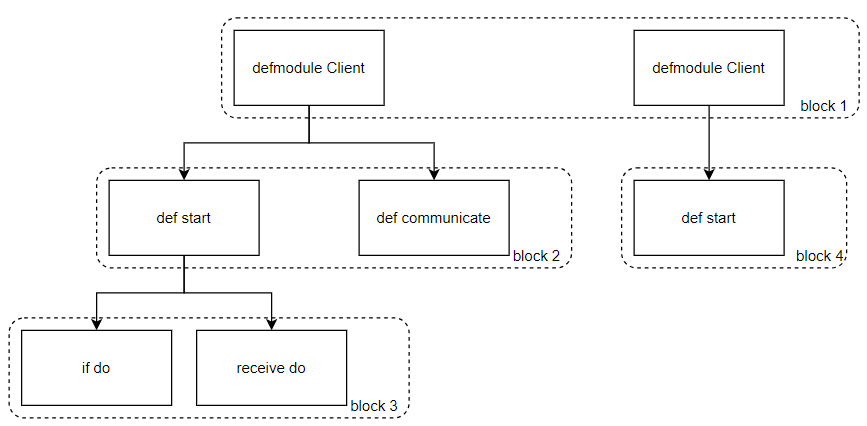
\includegraphics[width=0.8\textwidth]{images/sym_Table.png}
    \caption{An example of a scope hierarchy.}
    \label{fig:scope_hierarchy}
\end{figure}
\\ \\
\subsubsection{Traversal, Scoping and Variable Declarations}
Of course, that assumed a variable was not assigned to the child scope. In this case, we are required to track the execution of a scope in more detail. Let's first re-iterate Elixir's \texttt{match} operator and describe how the model generator handles it. Every expression in Elixir returns a value, and hence every expression can be matched on. We can match the entire return value of an expression to a single identifier, or use pattern matching to either have more granular control on how the return value is matched. We could also form guards for more complex checks used in conditional statements (such as \texttt{if} and \texttt{receive}). Elixir is a dynamically, strongly typed language. Dynamic typing enforces restrictions on the set of Elixir expressions we support. Strong typing helps type inference in model generation. In the intermediate representation (IR), a match is represented as either a declaration or an assignment. Given a declaration to an integer, we can infer the variable type and assign this in the symbol table. Now the variable is declared, any subsequent match in the same scope level is considered an assignment. If this assignment's inferred type does not align with the declared type, we raise an error.
\\ \\
If we now match on an expression that introduces a new child scope (such as a receive or if), we must explore every possible branch, determine the returning expression of the branch and use the relevant identifiers to assign the return value to the parent scope. To achieve this, the expression is traversed in using a depth-first search with a stack of lists. The stack manages the scope levels and the list manages the variable identifiers. Let's explore an example.
\begin{lstlisting}[language=Elixir, xleftmargin=.1\linewidth, caption={Representing variable declarations using the match operator}.]
    {player, action} = receive do
        {:move, player, direction} -> {player, "moved #{direction}"}
        {:attack, player, target} -> 
            send health, {target, -2}
            {player, "attacked #{target}"}
    end
\end{lstlisting}
In the example, we are matching on a tuple. We push $player$ and $action$ to the identifier list and then descend into the first guard (conditioned by the \texttt{:move} atom). This is a singular expression, so it must be the return value of this guard. We can peek the scope stack to access the list of variables, and iterate through them assigning the relevant values. Assuming this is a declaration, we also add the identifiers to the current scopes symbol table. We can mark direction as a $string$ as this is easily inferred, but we leave $player$ as $unknown$ until we can gather more information about the type. We now traverse the second branch. This follows the \texttt{block} construct, so we require pushing an empty list to the stack. We recursively apply this process until we reach the last expression in the block. Reaching the last expression, we can pop the stack (removing the child scope level) and then peek the stack to access the list of variables from the parent scope. We assign these using the same method, this time asserting the types align with the symbol table, or inferring more information about $unknown$ types if possible. \\ \\
\begin{figure}[h]
    \centering
    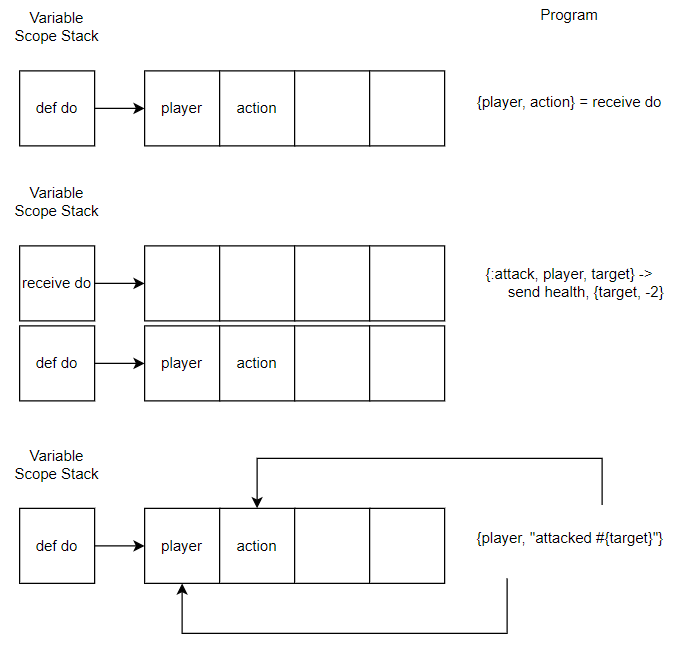
\includegraphics[width=0.8\textwidth]{images/var_stack.png}
    \caption{Example variable stack and identifier lists. The stack relates to the scope level, we push and pop as we traverse the receive guard. Only values waiting assignment are added to the identifier list.}
    \label{fig:scope_hierarchy2}
\end{figure}
\subsubsection{Functions, Type Specifications and Return Types}
Like the other constructs, functions introduce a new scope level. Multiple functions within a module and can be used to determine the control flow for a process. Before we discuss about the how functions are represented, we must quickly discuss types again. A correct LTLixir specification should provide type information for all function arguments and the return type. These properties are used to aid the type inference. The return type also determines how we model our function. If the return type is \texttt{:ok}, the function is non-returning, and we can treat the function as a standard sequential execution (but with its own local internal representation). If a return type is provided, we use a similar technique by recursively traversing expressions to determine all exit points of the function. 
\\ \\
Promela does not support functions. We model functions using Promela processes and rendezvous communication channels. To implement functions using our writer, we apply various techniques that mimick how Elixir functions behave. Firstly, the caller must declare a new rendezvous communication channel (using a buffer size of 0). A rendezvous channel has no buffer and hence communication over the channel is entirely synchronous. We also declare a new variable to store the return value of the function, typed using the type specification of the callee. We can now spawn a new process (a process mocking the function) and pass two imperative arguments alongside the arguments specified in the Elixir function. We first pass the channel, which acts as both a return value and signaling method for the function termination. We also pass a process identifier. All processes are identified by this process id; by passing this to the callee, the callee can take actions as if it were the parent process in communication. We then pass the remaining arguments as if we were making a true function call. The caller will now block until the callee sends a message over the signaling channel. The callee can proceed as normal, and by using the discussed traversal techniques, all exit points will send the final expression over the signaling channel. This approach easily extends to recursion, as the callee can spawn a new instance of itself and block until a signal is received.
\begin{figure}[h]
    \centering
    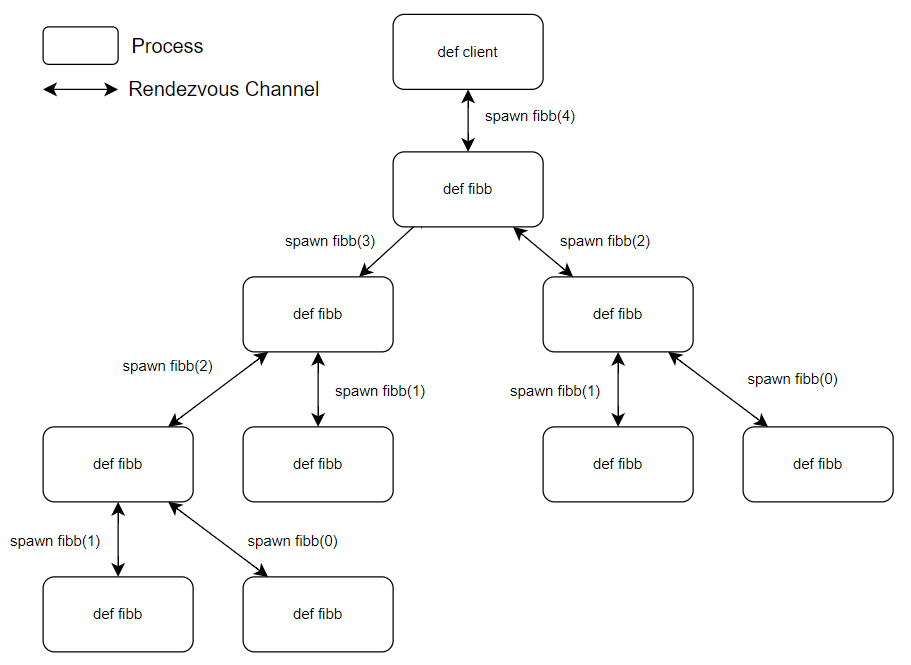
\includegraphics[width=0.8\textwidth]{images/function_call.png}
    \caption{An example of a recursive function call. In total, 9 processes are spawned to calculate the factorial of 4. Callers block until they rendezvous with callees. If we consider the call stack as a graph, it is traversed in a depth-first manner.}
    \label{fig:function_call}
\end{figure}
\subsection{Concurrent Memory Model} \label{sec:memory_model}
Now we have explored the basics of modelling Elixir programs, we extend the ideas to programs with multiple processes running concurrently. To correctly design a model of a concurrent Elixir system, there are a few core principles we must capture.
\begin{itemize}
    \item Spawning processes.
    \item Sending messages.
    \item Receiving messages.
    \item Bounding communication.
\end{itemize}
We will first explain how we model the spawning of a new process, before taking a deeper look into more interesting concurrency primitives as well as a memory model to extend the existing capabilities of Promela. The Verlixir IR for spawning processes resembles the Elixir spawn very closely. We capture a function that acts as the entry to the process which we can then model as a Promela process. As with a function call, we pass a process identifier to the new child process. In this case, the process identifier is a reserved identifier that signals to the new process to take a unique process identifier assigned automatically by the system. This is an important mechanism to ensure all parents are uniquely identifiable, which is crucial for communication. This process identifier can be captured in the caller's symbol table and used to communicate with the process.
\\ \\

\subsubsection{Actors, Mailboxes and Message Passing}
Once we have another process's identifier in our symbol table, we can begin communication between processes. Elixir implements this communication using the actor model, where each running process in the system is an actor that can send messages and receive messages using a mailbox. The mailbox can be considered a first-in-first-fireable-out queue. The IR must capture this ordering, otherwise it could misrepresent the execution of an Elixir program.
\\ \\
\subsubsection{Constructing Messages}
We begin by describing the design of a message. A message is comprised of two components, the \texttt{message type} and the \texttt{message body}. In Elixir, the message type is denoted with an atom, which the IR simply treats as a distinct type within the system. When the message type is used in the context of a send or receive it is added to a global set of message types. Tracking this set globally is important to model the entirety of the system, even if in reality, the message type has different meanings in local contexts. The message body consists of multiple message arguments. At this point, the IR does not refer to the message argument by its type but purely treats it as an argument that is expected to be passed in communication. We can store any primitive type within a message argument by inferring the type from the send or receive expression. If a type cannot be inferred in the context, we reserve a byte array to store the message argument, but to avoid this causing memory issues, we limit the size of the byte array to a small fixed size.
\\ \\
\subsubsection{Sending Message}
Now that we can construct a message, we can begin to model how messages can be sent and received. The IR keeps close to the mailbox system the actor-based implementation uses. Using the global message type set, we construct a per-process mailbox for each message type. The per-process mailboxes are constructed by passing a process identifier as an index on the channel, where the index aligns with the process identifiers we had previously been allocating. When a process sends a message, we triage which mailbox the message should be sent to using the message type and use the process identifier from the symbol table to index into the correct communication channel to attach the message.
\\ \\
\begin{figure}[h]
    \centering
    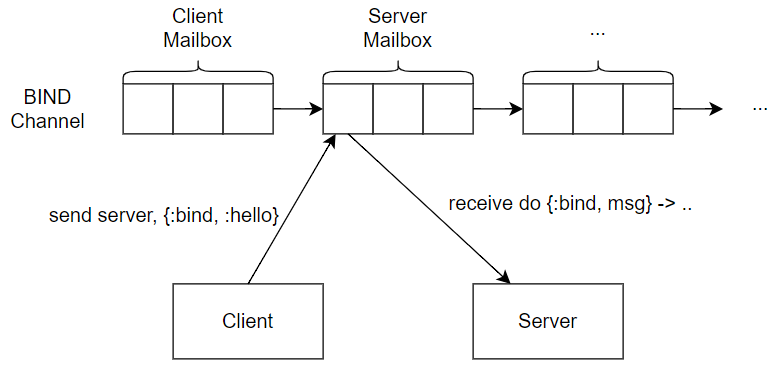
\includegraphics[width=0.8\textwidth]{images/promela_messages.png}
    \caption{An example of modelling the Elixir mailbox.}
    \label{fig:promela_mailbox}
\end{figure}
\\ \\
\subsubsection{Receiving Messages}
Receiving a message is a little more complex. We must now consider complex pattern matching in guard conditions. To begin pattern matching, we can again use the message type system to determine which mailbox to check. If more than just the message type is required in the pattern matching of a guard, we must preempt elements of the message body to determine which elements are important for pattern matching and which elements are identifiers that need assignments. In order to generate a model for the guards, we introduce a blocking statement consisting of multiple conditions. When one of the conditions is satisfied (i.e. a message has been pattern-matched) we stop blocking, execute the block relevant for the matched guard and then break out of the control structure. Before we can execute the block, we must assign all the remaining identifiers from the receive guard to the relevant values in the received message body. To do this, we first introduce a new dummy variable which is assigned the value of the entire message body. We can then access the dummy variable to assign the remaining identifiers from the guard. During the assignment, we have no indication of the type of the identifier. Hence, we can temporarily assign a message argument to the identifier, and extract the correct attribute from the message argument when we have more information about the type. A note on typing: the IR considers message types interchangeable with integers, hence comparisons can be made between the two which can be useful for matching. Sending messages is a non-blocking operation, unlike when we used rendezvous channels to model functions, if we send a message and do not care about receiving a returning message, we can continue executing the process body.
\\ \\
Unlike Elixir actors, Verlixir bounds multiple communication primitives. This is to ensure state explosion in the model checker is less likely to occur. As mentioned, we are strict in the bounding of byte arrays that can be passed as message arguments. We also only supply a small number of mailboxes per message type, furthermore, we bound the number of messages that can buffer in a per-process mailbox.
\subsubsection{Dynamic Memory Allocation}
Although not a direct fallout of the Elixir concurrency prinicples, Promela does not support dynamic memory allocation such as memory allocations (malloc) or memory de-allocations (free). This lack of support has lead to design choices in the generation of Elixir lists that if mishandled could lead to a mis-representation of Elixir concurrency in the target specification language. Immutability is a core feature of the Elixir runtime, hence the Elixir list operations introduce behaviours that must be carefully handled. For example, the \texttt{++} operator can be used to append or prepend elements to a list. If this is used to prepend, the operation is constant time, however the IR will represent this (as well as most list operations) as an operation in linear time. Let's explore the memory model to understand why. 
\\ \\
The IR introduces two structures to handle all list operations across the system. These structures are stored in the global scope context. The reason for this comes from Promela limitations. Promela supports statically sized arrays, and for good reasons regarding reducing state-space explosion, these arrays cannot be passed to other processes. Hence, an array's lifetime is limited to its scope. To get around this limitation, the two structures we introduce are called \texttt{memory} and \texttt{linked\_list}.
\\ \\
First we describe the design of \texttt{linked\_list}. Firstly, it is in fact not a traditional linked list, but it behaves similar as we can perform many operations on this structure that we could not perform on a statically size array. For example, we support prepending and appending in order to dynamically resize the list. In actualallity, none of these operations resize the list. A list has an upper bound in it's size, which is statically set for all model generation. Let's name this limit L.
\begin{lstlisting}[language=C, xleftmargin=.1\linewidth, caption={The structure of a list}.]
typedef linked_list {
    node vals[L];
}
\end{lstlisting}
For example for a limit, $10$, means the maximum number of elements that can be appended to the list is 10. The list starts as empty, this is handed by the \texttt{node} nested structure.
\begin{lstlisting}[language=C, xleftmargin=.1\linewidth, caption={Example of a list node typed `int'.}]
typedef node {
    int val;
    bool allocated;
}
\end{lstlisting}
A \texttt{node} stores a single value in a list, as well as a flag to indicate if the value has been allocated. Now, given a sequence of nodes, the order of the nodes represents the order of the Elixir list for all $true$ allocated nodes. For example, for a list, ls, $ls[0]$ and $ls[9]$ can be contiguous list elements if they are both allocated and there are no allocations inbetween.
\\ \\
Given this representation, we now see why all operations are in linear time. For example, for insertion (prepend or append), we must assign a pointer to a node and iterate through all nodes to find an unallocated node to insert into.
\\ \\
We now extend this implementation of a dynamically sized list to introduce dynamic memory. The implementation is very similar to how lists are implemented, we now introduce a new field to \texttt{linked\_list} called \texttt{allocated}. This represents the allocation of a list in memory. We now similarly introduce memory.
\begin{lstlisting}[language=C, xleftmargin=.1\linewidth, caption={Memory intermediate representation.}]
typedef memory {
    linked_list lists[10];
}
\end{lstlisting}
With this structure, we introduce a single globally defined instance of this structure named \texttt{\_\_memory}. All processes share this singular memory for their list allocations. All list operations are treated as a single, indivisible step so this does not introduce concurrent execution concerns. If an Elixir process declares a new list, the IR will represent this as a memory allocation. The model runtime will iterate through all the lists in memory to find an unallocated list, as return this as a pointer to the process. Of course, as dynamic memory allocations is not supported in Promela, this $pointer$ is generated as an \texttt{int}, which indexes into memory. 
\\ \\
Finally, with all these definitions in place we can finally support the passing of Elixir lists as function arguments. When we detect a function call, or \texttt{send} expression passing a list, we first allocate a pointer to a new location in memory, we then copy all the values from the list into the new allocated list and then pass the pointer as an argument. With this mocked memory in place, we can now support Elixir lists and operations on lists, we will discuss a few of these operations next.
\\ \\
\subsubsection{Iteration and Higher Order Functions}
Promela supports for loops, but for our custom dynamic memory these do not suffice to represent Elixir for comprehensions. Using a similar approach we used to append list elements, a for comprehension can be represented as a linear scan through all \texttt{linked\_list} elements to find the allocated elements, and then only applying the comprehension body to these. We can introduce temporary dummy variables to represent Elixir's \texttt{<-} operator. If we want to match on a for comprehension, we must also introduce a pointer into a second \texttt{linked\_list} which tracks new allocations into the matched block independently of the scan through an existing list. A for comprehension over an Elixir range construct, \texttt{n..m}, can be represented with a for loop.
\\ \\
A map operation (such as from the \texttt{Enum} Elixir library) are represented similarly to for comprehensions in the IR. Instead of inlining the body, in order to hold a more fair representation of the Elixir program, dummy anonymous processes are stored to represent higher-order functions.
\\ \\
As a closing note on memory, we describe the representation of randomness. Again, Promela does not inherently support randomness which has influenced the IR design. To represent a function such as \texttt{random} from the \texttt{Enum} library, we represent this using multiple truth conditions that can be selected from non-deterministically. One of these conditions will return an allocated list element and one will increment the current list pointer. To ensure termination, if we point to the end of the list before returning a value, we simply return the last allocated value we saw. This is not true randomness, and is not fair to all elements in the list hence random operations are strongly discouraged in LTLixir, but are theoretically supported.
\\ \\
Note that as Promela does not support functions, when we generate a model, all of these Elixir functions are in-lined into the process body. Any reference to a function $return$ is actually simply generated as an assignment.

\subsection{Supporting LTLixir} \label{sec:supporting_ltl}
In section \ref{sec:specification_language} we discussed how Elixir was extended to support inline specifications. We now describe how these are modelled in the IR and generated in Promela.
\\ \\
\subsubsection{System Entry}
The \texttt{@vae\_init} LTLixir attribute represents an entry point to the system. We represent this using a flag in the IR for each process, controlling if the process should be running in the first state of the model or not.
\\ \\
\subsubsection{Type Specifications}
A \texttt{@spec} attribute is parsed when parsing a function definition. For each argument being parsed when creating a new function in the IR, we insert a new symbol table entry using the type provided in the type specification. The return type is a special case of this as it could be the non-returning \texttt{:ok} type. If this is received, we insert a reserved non-returning type into the symbol table, and interface with this by supporting a \texttt{table.returning\_function() $\rightarrow$ boolean} call to determine if a function if returning or not. If a function is non-returning, it would be an error to attempt to look up the type of the function in any context. If a function is returning, we must ensure all expressions which are returning (i.e. last in a block) write to the rendezvous channel, as discussed in section \ref{sec:sequential_execution}.
\\ \\
\subsubsection{Concurrency Parameters}
A \texttt{@params} attribute also instruments the IR of a function. For all of the parameters in the tuple of identifiers, we mark these before continuing with storing the remainder of the function. When a declaration of one of these identifers is found in an expression, we avoid the usual handling of this and instead assign a dummy value \texttt{\_\_PARAM} to the identifer. This dummy value is used by the model generator to create multiple configurations of a single model, which will be discussed more in section \ref{sec:simulation_verification}.
\\ \\
\subsubsection{Linear Temporal Time Formulae}
The final attribute is \texttt{@ltl}. When an LTL formula is parsed, we create a set of all identifers (or predicates) present in the formula. We first instrument the function body by marking all these identifers as LTL identifers. When we detect the declaration of an LTL identifer to an expression, we extract this declaration out of the function and move it to the global context. Internally, we now consider this a system property as opposed to a property of a single process. When we have extracted all LTL identifer declarations, we can handle the conditions of the LTL formula, such as the temporal properties. We construct formulae from the system properties using the same operators the user defined in the attribute. We finally mark these formulae as LTL formulae in the IR, which means the Promela model generator can create LTL properties from them to be constructed with the rest of the state-space during verification.
\\ \\
\subsubsection{Predicates}
Similarly to LTL properties, any predicates are tracked in a similar way. Any identifers that construct a predicate must be extracted to the global context and flagged as system properties. We also globally define the predicates using the system properties in order to ensure they are valid within an LTL formuae.
\\ \\
\subsubsection{Verifiable Functions}
The \texttt{defv} construct is handled as the the other function definitions are as described in section \ref{sec:sequential_execution}. Verifiable functions are still internally represented as processes, however we now also extract the pre- and post-conditions from the definition. A pre-condition instruments a function-body by inserting an additional condition that's truth is evaluated before the rest of the function body. A post-condition flag is set in the functions definition in the event one is parsed. When a post-condition flag is set, we ensure to instrument all returning expressions of a function to assert the truth of the post-condition. As in the IR, functions actually write to a rendezvous channel instead actually returning, we perform this violation check after the return point of a function. When the verifier is ran on a model, every state in the state-space is exhausitvely checked, hence any possible evaluation of a pre- or post-condition will be exhaustively checked in the verification process. This provides better assurance than relying on the condition checks during the Elixir runtime.

\section{Simulation and Verification} \label{sec:simulation_verification}
We have now explored the intermediate representation constructed by Verlixir, alongside some implementation details specific to using Promela as a target language. This section will describe the remainder of the Verlixir design, which touches on simulation, verification, generating multiple models and using Spin as a target model checker. The vanilla execution of the Verlixir executable will produce a single Promela model for a given input LTLixir specification. For Verlixir to produce outputs, it should be executed with a flag to set the mode: $\{-s, -v, -p\}$ for simulation, verification or parameter exploration. The flags determine how the Spin model checker is ran.
\\ \\
If $-s$ is passed, Spin is ran in vanilla simulation mode. If $-v$ is passed, Verlixir will first determine the existence of LTL properies within the model. For each LTL property, we run an instance of Spin specifying the LTL property we want to evaluate. We do this using Spin's $-search$ parameter, which will generate and run the verifier from the model. In the case we do not detect an LTL property, we use $-search$ to check for the existence of deadlocks or non-progress cycles (livelocks). If $-p$ is passed, multiple models are generated instead of one, and all of these are checked as if $-v$ was passed for each.
\subsection{Simulation}
Simulation mode will use the Spin scheduler to execute a single execution through the generated state-space. A simulation can timeout in the case of a deadlock. If a timeout is produced, we inform the user of the timeout but do not provide further information as that is left for verification mode. Elixir calls to the \texttt{IO} library can be re-produced in simulation mode as we display them to the user if they are executed. These are not as proficient as using \texttt{IO} in the Elixir runtime. Simulation mode can be more beneficial than examining the output of running an Elixir program, as the scheduler takes enabled transitions based on the current state, whereas the Elixir scheduler, runs in real-time which can result in a process interleaving never being observed.
\subsection{Verification}
Verification mode will run the Spin verifier. If an error is detected, the output is captured by the Verlixir error profiler, which triages the issue to generate relevant outputs for the user to digest. For example, if a non-acceptance cycle is produced by Spin, Verlixir captures this and reports to the user that either an LTL property was violated (liveness property) or the system is potentially livelocked. Verlixir will report the entire trace that lead to this cycle, showing which process was responsible for a transition between states as well as reading from the Elixir module the line of Elixir code that lead to that transition. 
\\ \\
\subsubsection{Reporting Violations}
The mapping between Elixir expressions and how they are modelled is not a one-to-one mapping of line-numbers. Instead a single Elixir expression can result in multiple Promela expressions and multiple states in the state-space Spin traverses. Still, all the relevant Elixir expressions are captured and reported in the trace produced. For this error, Verlixir will also report the cycle that lead to non-terminating processes. It will report where the cycle begins, then give a trace of executed Elixir lines and which function exectued them. The error profiler also captures and reports the processes which have terminated, or a blocking expression (such as a receive with no accepting guards). For a given model $M$, the profiler can determine the following truth conditions for the specification $\phi$. If the specification holds for an initial state, $S_i$, we have $(M, S_i) \models \phi$. If the specification holds for all initial states, the specification is valid: $M \models \phi$. The error profiler may report a violation, in which case for a violating specifiation $\phi _v$ we have $(M, S_i) \models \phi _v$. For example, deadlocks, non-accept cycles, out-of-memory, assertion violations are possible violating specifications all represented by $\phi _v \in \{\phi _{dl}, \phi _{cycle}, \phi _{memory}, \phi _{assert}\}$. In the event that $M \models \phi _{memory}$, we could re-run the verification process using directives to reduce memory usage. If this is required, Spin will no longer perform an exhaustive search. If the specification is true under these conditions, we can only say the model partially models the specification, $(M, S_i) \models \phi _p$. Non-exhaustive search should only be applied as a last resort, if it is infeasible to perform verification by reducing the system complexity and can be performed using the $-r$ flag. 
\\ \\
\subsubsection{Fairness}
Similarly, in the event $M \models \phi _{cycle}$, it may be useful to introduce weak fairness to the system. Weak fairness can be applied by passing the $-f$ flag when in verification mode. Other flavours of fairness should be introduced using LTL formulas. If the weak fairness flag is active, scheduling decisions will consider how process-level non-determinism is resolved. For example, if a non-progress cycle is detected by a single process infinitely executing even when there are other active processes that are not being scheduled, by re-running the verifier with weak fairness applied, infinitely enabled transitions will eventually be scheduled to be taken. This may instead report a new error, consisting of a fair non-progress cycle, or even avoid the non-progress cycle entirely.  
\subsection{Parameterization}
The Verlixir IR passes all detected parameters to the Verlixir model runner. The model runner is reponsible for generating multiple models depending of the number of paramters provided, $N$ and the range of search values, $M$, which can be parsed as a command line argument using $-p\text{ }M$. The model runner generates a total of $M^N$ Promela models. All of these models are ran in $-search$ mode and violations are reported. Verlixir reports an acceptance score, $\alpha$, determing how many of the model were accepted by the verifier: $\alpha \coloneq 1 - \frac{|V|}{M^N}$, where $V$ are violating models. After outputting $\alpha$, we note all the elements of $V$ so the user can generate a trace for the violation using verification mode.

\section{Modelling Paxos}
We will now demonstrate the model generation process for a larger example, the basic Paxos algorithm. A thorough explanation of the problem will be discussed in section \ref{sec:Paxos}. For now, we will just concern ourselves with the syntax of the Elixir program and how it is parsed and translated into Promela.
\\ \\
The entire program is large, so we will just look at a single Elixir $defmodule$. In particular, we will look at the $learner$ module. When the system is distributed, the $learner$ could be an Elixir node, or an Elixir process. For our model, it does not matter. We will now take a look at the Elixir implementation of one of the functions of the learner, $wait\_learned$, focusing primarily on the syntactic elements.
\\ \\
\begin{lstlisting}[language=Elixir, xleftmargin=.05\linewidth, caption={A function from the $learner$ module}.,label = lst:learner]
@spec wait_learned(list(), integer(), integer()) :: :ok
@ltl """
[]((p->!<>q) && (q->!<>p))
<>(r)
[](s)
"""
def wait_learned(acceptors, p_n, learned_n) do
    predicate p, final_value == 31
    predicate q, final_value == 42
    predicate r, final_value != 0
    predicate s, final_value == 0 || final_value == 31 || final_value == 42

    if p_n == learned_n do
        for acceptor <- acceptors do
            send acceptor, {:terminate}
        end
    else
        receive do
            {:learned, final_value} ->
            IO.puts("Learned final_value:")
            IO.puts(final_value)
        end
        wait_learned(acceptors, p_n, learned_n + 1)
    end
end
\end{lstlisting}
Listing \ref{lst:learner} shows an Elixir function, $wait\_learned$. The function specifies some LTL properties, using the multi-line LTL syntax. The LTL properties rely on the predicates defined in the function body. The function also receives some arguments. In the body, we see conditional branch, where one branch involves a for comprehension through a list performing some message sending. The other branch receives a value. At the end of the $else$ condition, we recurse. Let's now break down the Promela model.
\\ \\
\begin{lstlisting}[language=Promela, xleftmargin=.1\linewidth, caption={Promela function definition}., label=lst:func_def]
#define p ((final_value == 31))
#define q ((final_value == 42))
#define r ((final_value != 0))
#define s ((((final_value == 0) || (final_value == 31)) || (final_value == 42)))

proctype wait_learned (int acceptors;int p_n;int learned_n;chan ret;int __pid;int __ret_f) {
    chan ret1 = [1] of { int }; 
    atomic{
        if
        :: __pid == - 1 -> __pid = _pid;
        :: else -> skip;
        fi;
    }
\end{lstlisting}
Listing \ref{lst:func_def} shows the first translation result of Promela from the Elixir function. Firstly, we see the predicates are pulled from the body and placed into the global context.
\\ \\
The function is translated to a process type, named $wait\_learned$. The process receives the same arguments as the Elixir function, using the type specification to type the arguments. Additionally, we receive some meta-arguments $\_\_pid$ and $\_\_ret\_f$. The first line of the function body creates a channel, named $ret1$. Channels of this nature will be used in function calls, likely later in the body.
\\ \\
Finally, we see an $atomic$ block, which perform a check on the received $\_\_pid$. If the process id passed is $-1$, we assign a new process id from the process scheduler. Otherwise, we continue to act as the caller, by retaining the passed process id.
Next, we look at the first branch of the Elixir $if$ statement. In particular, we will look at the for comprehension.
\begin{lstlisting}[language=Promela, xleftmargin=.1\linewidth, caption={Promela if statement and for comprehension}., label=lst:for]
if
:: (p_n == learned_n) -> 
    atomic {
        __list_ptr_old = __list_ptr;
        __list_ptr = 0;
        __list_ptr_new = 0;
        do
        :: __list_ptr >= LIST_LIMIT || __list_ptr_new >= LIST_LIMIT -> 
            __list_ptr = __list_ptr_old;
            break;
        :: else -> 
            if
            :: LIST_ALLOCATED(acceptors,__list_ptr) -> 
                int acceptor;
                acceptor = LIST_VAL(acceptors,__list_ptr);
                atomic {
                    MessageList msg_0;
                    __TERMINATE!!acceptor,TERMINATE,msg_0; 
                }
                ;
                __list_ptr_new++;
                __list_ptr++;
            :: else -> __list_ptr++;
            fi
        od
    }
\end{lstlisting}
Listing \ref{lst:for} shows the translation for the $if$ statement. Each condition in the $if$ is determined with a (::) operator. In this listing, we just have the first condition, the $else$ will be seen in a later listing. 
\\ \\
Next, we have the translation of the for comprehension. This is wrapped in an atomic block, as it relies on accessing shared memory. It looks daunting, but all that is taking place is a linear scan through the list. We check each element, determine if it has been assigned to a value, and if it has, then the comprehension body (lines 14 through 19) is executed with the list element.
\\ \\
In this case, the comprehension body is a $send$. To send, we pack the message elements into structure, and then send this data to the channel matching our $terminate$ atom, and the mailbox matching $acceptor$.
\\ \\
Now let's look at the $else$ condition.
\begin{lstlisting}[language=Promela, xleftmargin=.1\linewidth, caption={Promela receive and recursion}., label={lst:else}]
:: else -> 
    MessageList rec_v_5;
    do
    :: __LEARNED??eval(__pid),LEARNED,rec_v_5 -> 
        final_value = rec_v_5.m1.data2;
        printf("Learned final_value:\n");
        printf("final_value\n");
        break;
    od;
    int __temp_cp_arr_2;
    __copy_memory_to_next(__temp_cp_arr_2,acceptors);
    int __ret_placeholder_1;
    run wait_learned(acceptors,p_n,learned_n + 1,ret1,__pid,1);
    ret1?__ret_placeholder_1;
fi;
\end{lstlisting}
Listing \ref{lst:else} shows the translation of the $else$ condition. Again, this is guarded by a (::) operator. We do two things here: first we receive a message and then we recurse.
\\ \\
The receive only has one guard. We translate this guard by reading from the $learned$ channel, looking into our own mailbox (marked by $\_\_pid$). The data we read from the channel is read into $rec\_v\_5$, which we unpack into the relevant variables.
\\ \\
Secondly, we make a recursive function call. As one of the arguments passed is a list, we must ensure we pass the list by value. To do this, we get a new pointer from memory, and copy the values from our local list into the new memory location.
\\ \\
We next create a value to store the returned value from the recursive call. Actually, in this case the function's type definition marked the function as `non-returning'. We recursively call the function by spawning a new instance of the process type. We pass the parameters, as well as the relevant meta-arguments. In this case, the meta-arguments are:
\begin{itemize}
    \item The channel to send the return value to, $ret1$. This was defined at the beginning of the function body.
    \item We pass our own process id, so the spawned function can continue to take actions on our behalf.
    \item We pass $1$. $1$ marks a non-returning function.
\end{itemize}
We then wait to read on $ret1$ to rendezvous with the callee.
\\ \\
Let's finally look at the remaining translated code.
\begin{lstlisting}[language=Promela, xleftmargin=.1\linewidth, caption={Translation of LTL properties}., label={lst:final}]
    atomic{
        if
        :: __ret_f -> ret!0;
        :: else -> skip;
        fi;
    }
}


ltl ltl_1 { []((p -> ! <> q) && (q -> ! <> p)) };
ltl ltl_2 { <> (r) };
ltl ltl_3 { [](s) };
\end{lstlisting}
Listing \ref{lst:final} shows the remainder of the translated code. To end the function, we have a final $atomic$ block. Within this block, we check the value of the passed $\_\_ret\_f$ value. If this is $1$, the function is non-returning. To handle the resolution of the call stack, we propagate a ghost $0$ through the return channels. If it was a returning function, the return would already have been handled, and hence we can $skip$.
\\ \\
Finally, after the function and back in the global context, we define our LTL properties. We split the multi-line property into multiple properties so they can be checked in parallel. They rely on the predicated defined, which were defined in the global context as they are properties of the system, not a single process.
\\ \\
\section{Summary}
This chapter has discussed some core design concepts behind LTLixir and Verlixir. We first looked at a high-level overview of where the tools fit into a wider toolchain and gave a basic introduction to their architecture. We saw how Elixir was extended using metaprogramming to support inline specifications. We then introduced the core techniques essential to constructing an intermediate representation of an LTLixir specification as well as how Promela can be used as a target modelling language for Elixir systems. Finally, we looked at how Verlixir interacts with the model checker Spin to simulate and verify programs while capturing traces of Elixir programs. We will now evaluate the effectiveness of this tooling.
